\documentclass[UTF8,11pt]{ctexart}

\usepackage[a4paper,margin=2.2cm]{geometry}
\usepackage{graphicx}
\usepackage{subcaption}
\usepackage{booktabs}
\usepackage{longtable}
\usepackage{array}
\usepackage{amsmath}
\usepackage{xcolor}
\usepackage{hyperref}
\usepackage{enumitem}

\graphicspath{{figures/}}
\hypersetup{
  colorlinks=true,
  linkcolor=blue!60!black,
  urlcolor=blue!60!black,
  citecolor=blue!60!black
}
\setlist[itemize]{leftmargin=1.8em,itemsep=0.2em,topsep=0.3em}

\title{IVOCT 钙化分割阶段性实验报告}
\author{CN\_seg 项目}
\date{2026-04-24}

\begin{document}
\maketitle

\begin{abstract}
本文档汇总当前阶段 IVOCT 钙化分割实验的最优结果、实验设置、可视化表现和后续计划。
当前主线方案为 \textbf{MAE encoder + Conv decoder}，采用 4 名患者的
leave-one-patient-out cross validation (LOPO-CV) 进行验证。重跑后的最优
baseline 在 4 折上取得 Mean Dice $0.5212 \pm 0.1424$。阈值扫描显示，
统一阈值 $0.3$ 仍是当前最合适的全局阈值。针对最弱折 P002 的单独改动能够带来
局部提升，但会降低整体 LOPO 表现，因此目前不作为正式主线。考虑到后续还有 14 名
患者数据待加入，当前建议保留该 baseline 作为阶段性结果，并在新增数据到位后重新
评估泛化能力与训练策略。
\end{abstract}

\section{研究目标与当前阶段}

本阶段目标是在已有 MAE 预训练特征的基础上，建立一套可复现的 IVOCT 钙化区域分割
baseline。当前数据量较小，仅包含 4 名患者，因此实验重点不是追求对现有样本的过度
拟合，而是形成一个清晰、可复现、可作为后续扩展对照的基线。

当前报告回答三个问题：

\begin{itemize}
  \item 当前最优分割策略是什么；
  \item 在 4 名患者 LOPO-CV 上的分折表现如何；
  \item 在剩余 14 名患者加入前，是否有必要继续围绕当前 4 名患者调参。
\end{itemize}

\section{数据与验证设计}

当前实验包含 4 名患者，记为 P001、P002、P003、P004。验证方式为 LOPO-CV，
每次留出 1 名患者作为验证集，其余 3 名患者作为训练集。该设置更接近患者级泛化评估，
比随机划分更能反映模型跨患者迁移能力。

\begin{table}[htbp]
\centering
\caption{LOPO-CV 数据划分}
\label{tab:splits}
\begin{tabular}{cll}
\toprule
Fold & 训练患者 & 验证患者 \\
\midrule
0 & P002, P003, P004 & P001 \\
1 & P001, P003, P004 & P002 \\
2 & P001, P002, P004 & P003 \\
3 & P001, P002, P003 & P004 \\
\bottomrule
\end{tabular}
\end{table}

根据本次评估日志，各验证患者的样本数分别为 P001 10 张、P002 14 张、P003 8 张、
P004 11 张。样本量仍然有限，因此本文将当前结果视为阶段性 baseline，而不是最终
定型方案。

\section{模型与训练策略}

当前主线模型由两个部分组成：

\begin{itemize}
  \item MAE encoder：使用既有预训练权重，并在分割训练中冻结；
  \item Conv decoder：在分割任务上训练，用于输出像素级预测。
\end{itemize}

该策略的优点是训练成本较低，且能复用已有无监督/自监督预训练特征。训练中使用
中心 ROI 裁剪、统一输入尺寸和固定随机种子，以保证实验可复现。

\begin{table}[htbp]
\centering
\caption{主线训练配置}
\label{tab:config}
\begin{tabular}{ll}
\toprule
项目 & 配置 \\
\midrule
模型结构 & MAE encoder + Conv decoder \\
输入尺寸 & $256 \times 256$ \\
ROI 裁剪比例 & 0.86 \\
Patch size & 8 \\
Embedding dim & 384 \\
Encoder depth & 12 \\
Attention heads & 6 \\
Encoder 状态 & 冻结 \\
Epochs & 300 \\
Batch size & 4 \\
Decoder learning rate & $1 \times 10^{-3}$ \\
Weight decay & 0.05 \\
Warmup epochs & 5 \\
AMP & 开启 \\
随机种子 & 42 \\
\bottomrule
\end{tabular}
\end{table}

训练脚本为 \texttt{seven/seg/train\_seg.py}，服务器运行目录为
\texttt{/root/CN\_seg\_baseline/seven/seg}。本次主线结果文件为：

\begin{center}
\texttt{/root/CN\_seg\_baseline/seven/seg/logs/results\_lopo\_20260424\_004401.json}
\end{center}

\section{评价指标}

报告主要使用 Dice 和 IoU 评价分割重叠程度，并辅助记录 sensitivity 与 specificity。
设 $TP$、$FP$、$FN$、$TN$ 分别为真阳性、假阳性、假阴性和真阴性，则：

\begin{align}
\mathrm{Dice} &= \frac{2TP}{2TP + FP + FN}, \\
\mathrm{IoU} &= \frac{TP}{TP + FP + FN}, \\
\mathrm{Sensitivity} &= \frac{TP}{TP + FN}, \\
\mathrm{Specificity} &= \frac{TN}{TN + FP}.
\end{align}

Dice 是本文最主要的比较指标。对于钙化区域这类小目标分割任务，Dice 对漏检和过分割
都比较敏感，因此适合作为当前阶段的主指标。

\section{主线实验结果}

当前 reproduced baseline 的 LOPO-CV 平均 Dice 为：

\begin{center}
\Large
$0.5212 \pm 0.1424$
\end{center}

分折结果见表~\ref{tab:fold-results}。P003 与 P004 表现较好，P001 居中，
P002 为当前最弱折。

\begin{table}[htbp]
\centering
\caption{Baseline LOPO-CV 分折结果}
\label{tab:fold-results}
\begin{tabular}{ccccc}
\toprule
Fold & 验证患者 & Best epoch & Dice mean & IoU mean \\
\midrule
0 & P001 & 177 & 0.5288 & 0.3746 \\
1 & P002 & 168 & 0.2861 & 0.1805 \\
2 & P003 & 52  & 0.6323 & 0.4643 \\
3 & P004 & 94  & 0.6374 & 0.4775 \\
\midrule
\multicolumn{3}{r}{Mean $\pm$ Std} & $0.5212 \pm 0.1424$ & -- \\
\bottomrule
\end{tabular}
\end{table}

从患者维度看，当前主要瓶颈不是所有折都偏低，而是患者间差异较大。尤其是 P002，
其 Dice 明显低于其余三个患者，说明当前模型已经具备一定分割能力，但患者级泛化仍是
后续需要重点关注的问题。

\section{可视化结果}

图~\ref{fig:fold-vis} 展示了 4 个 fold 在 best epoch 下的可视化结果。每个子图中
包含输入 IVOCT 图像、模型预测和人工标注，用于直观检查模型预测区域与标注区域的
对应关系。

\begin{figure}[htbp]
\centering
\begin{subfigure}{0.48\textwidth}
  \centering
  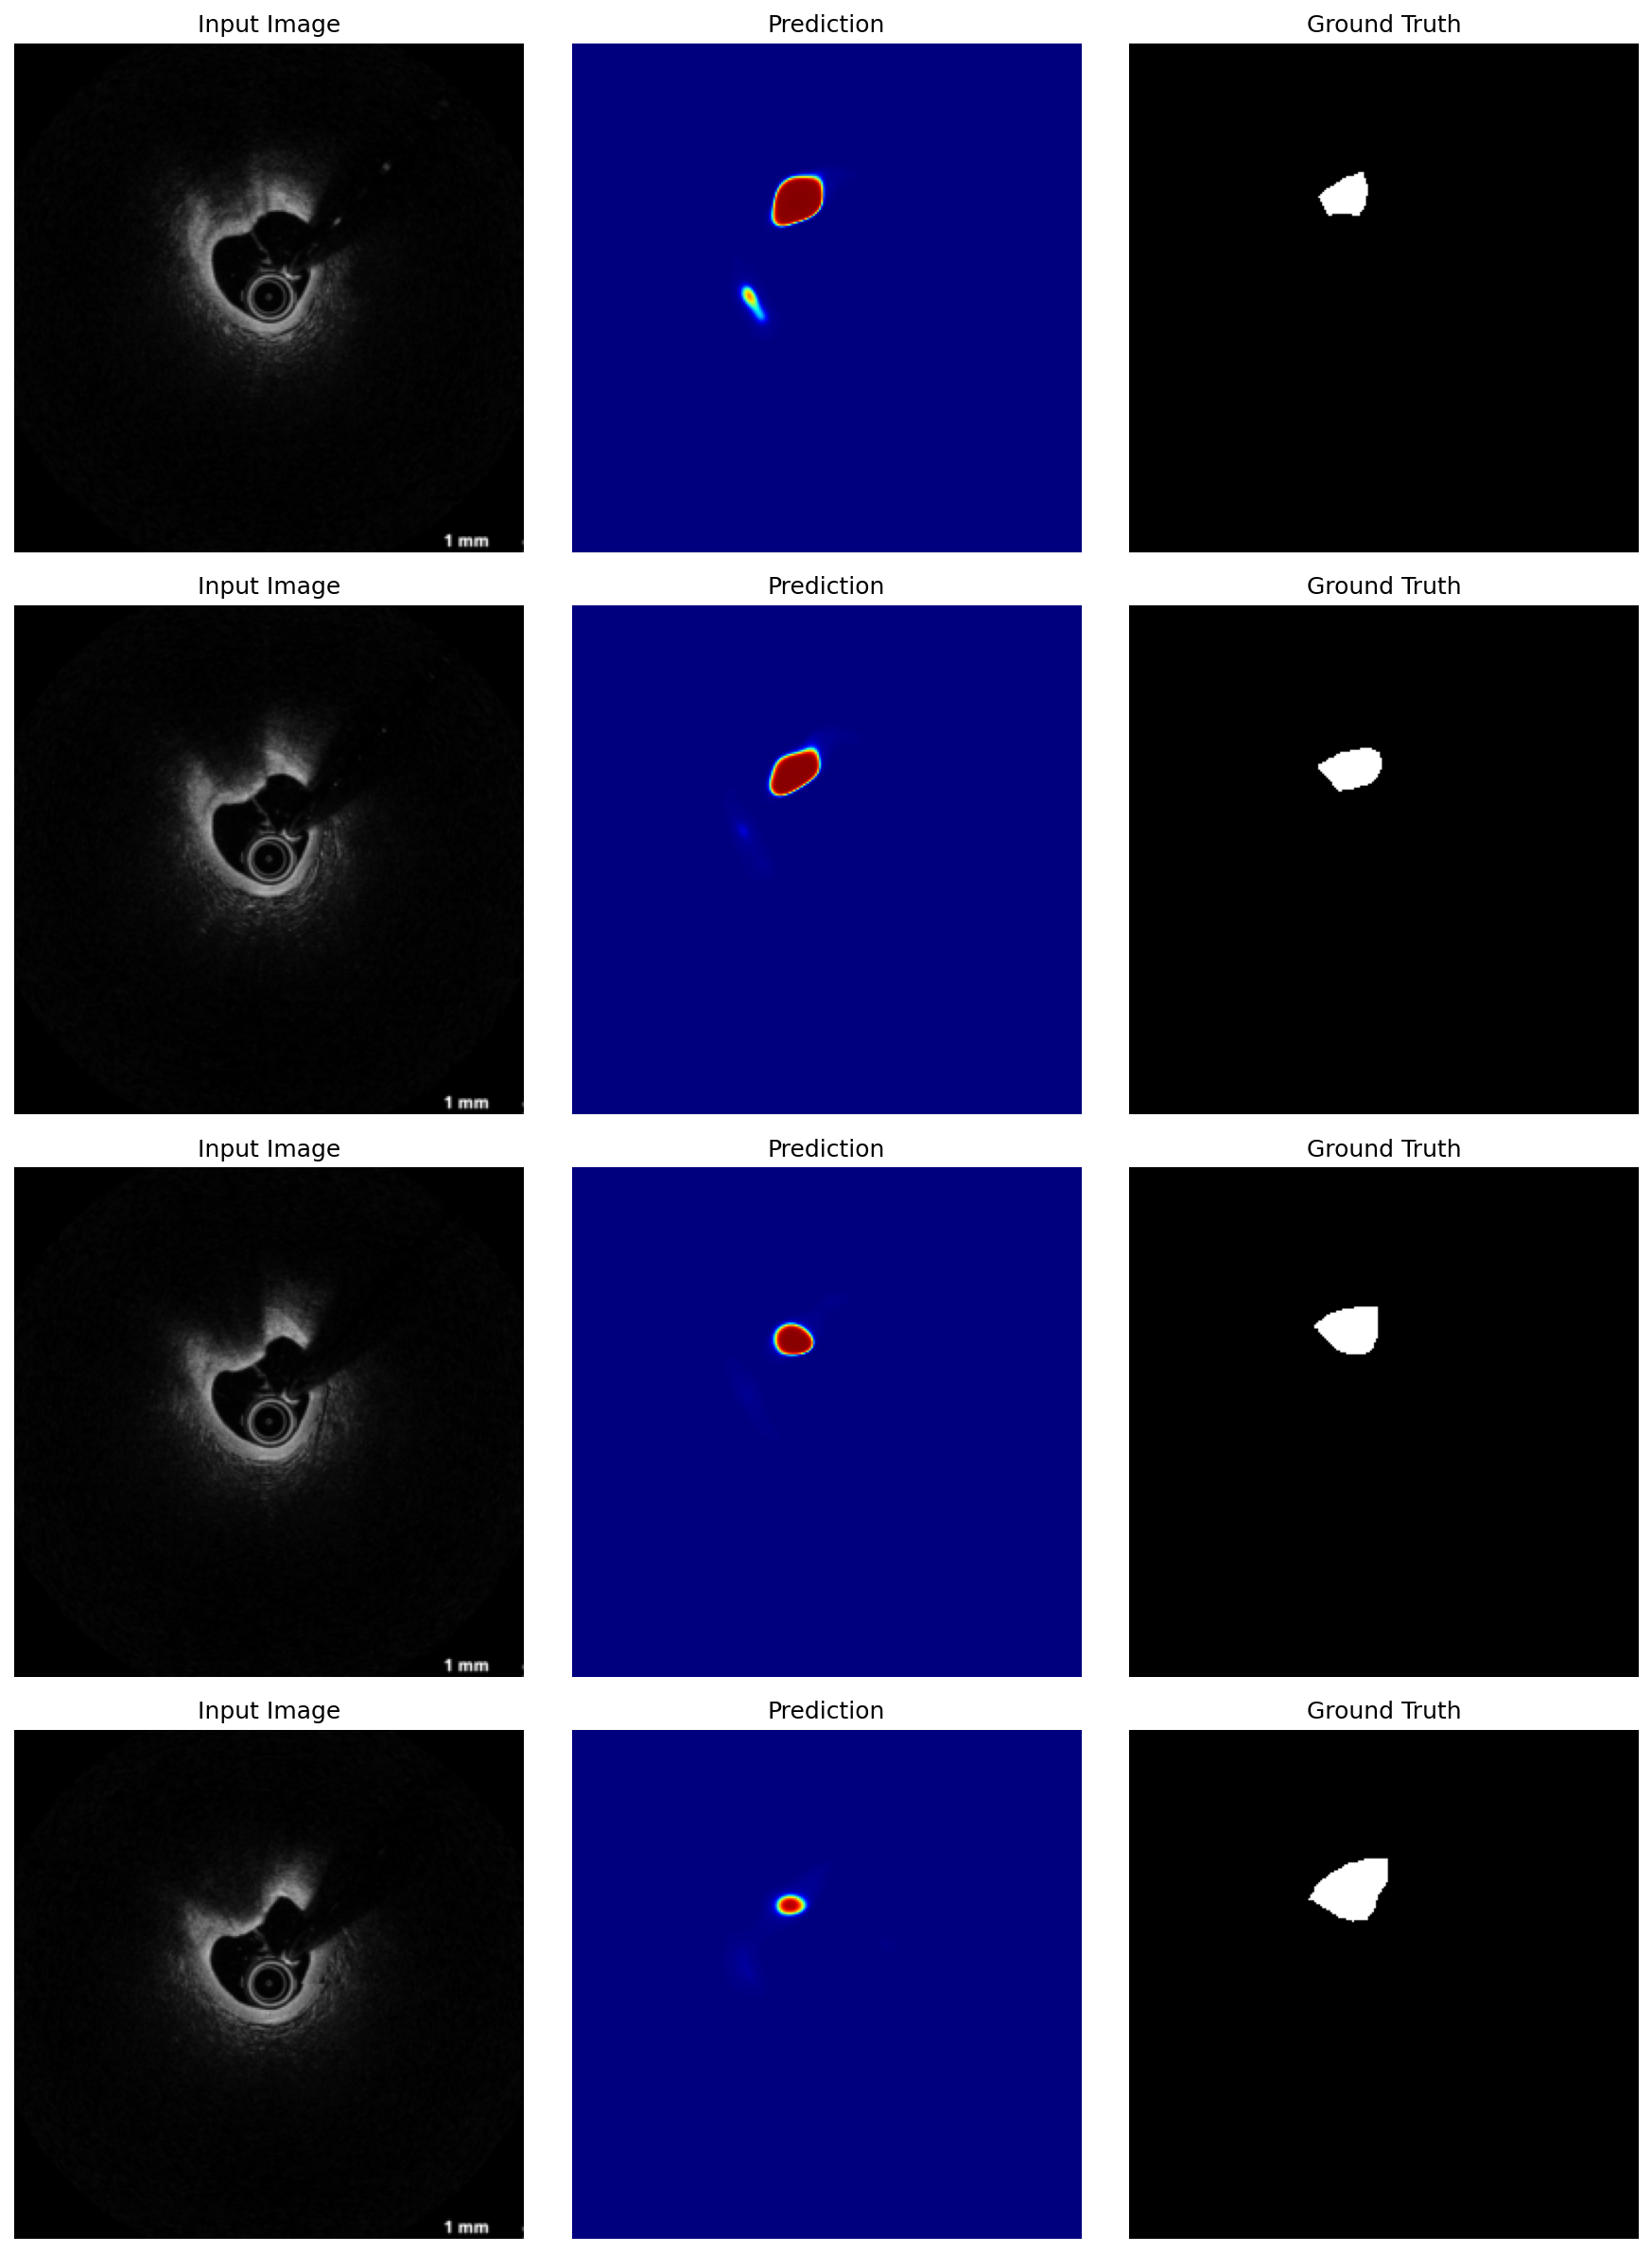
\includegraphics[width=\linewidth]{fold_0_best_epoch_177.png}
  \caption{Fold 0, val=P001, Dice=0.5288}
\end{subfigure}
\hfill
\begin{subfigure}{0.48\textwidth}
  \centering
  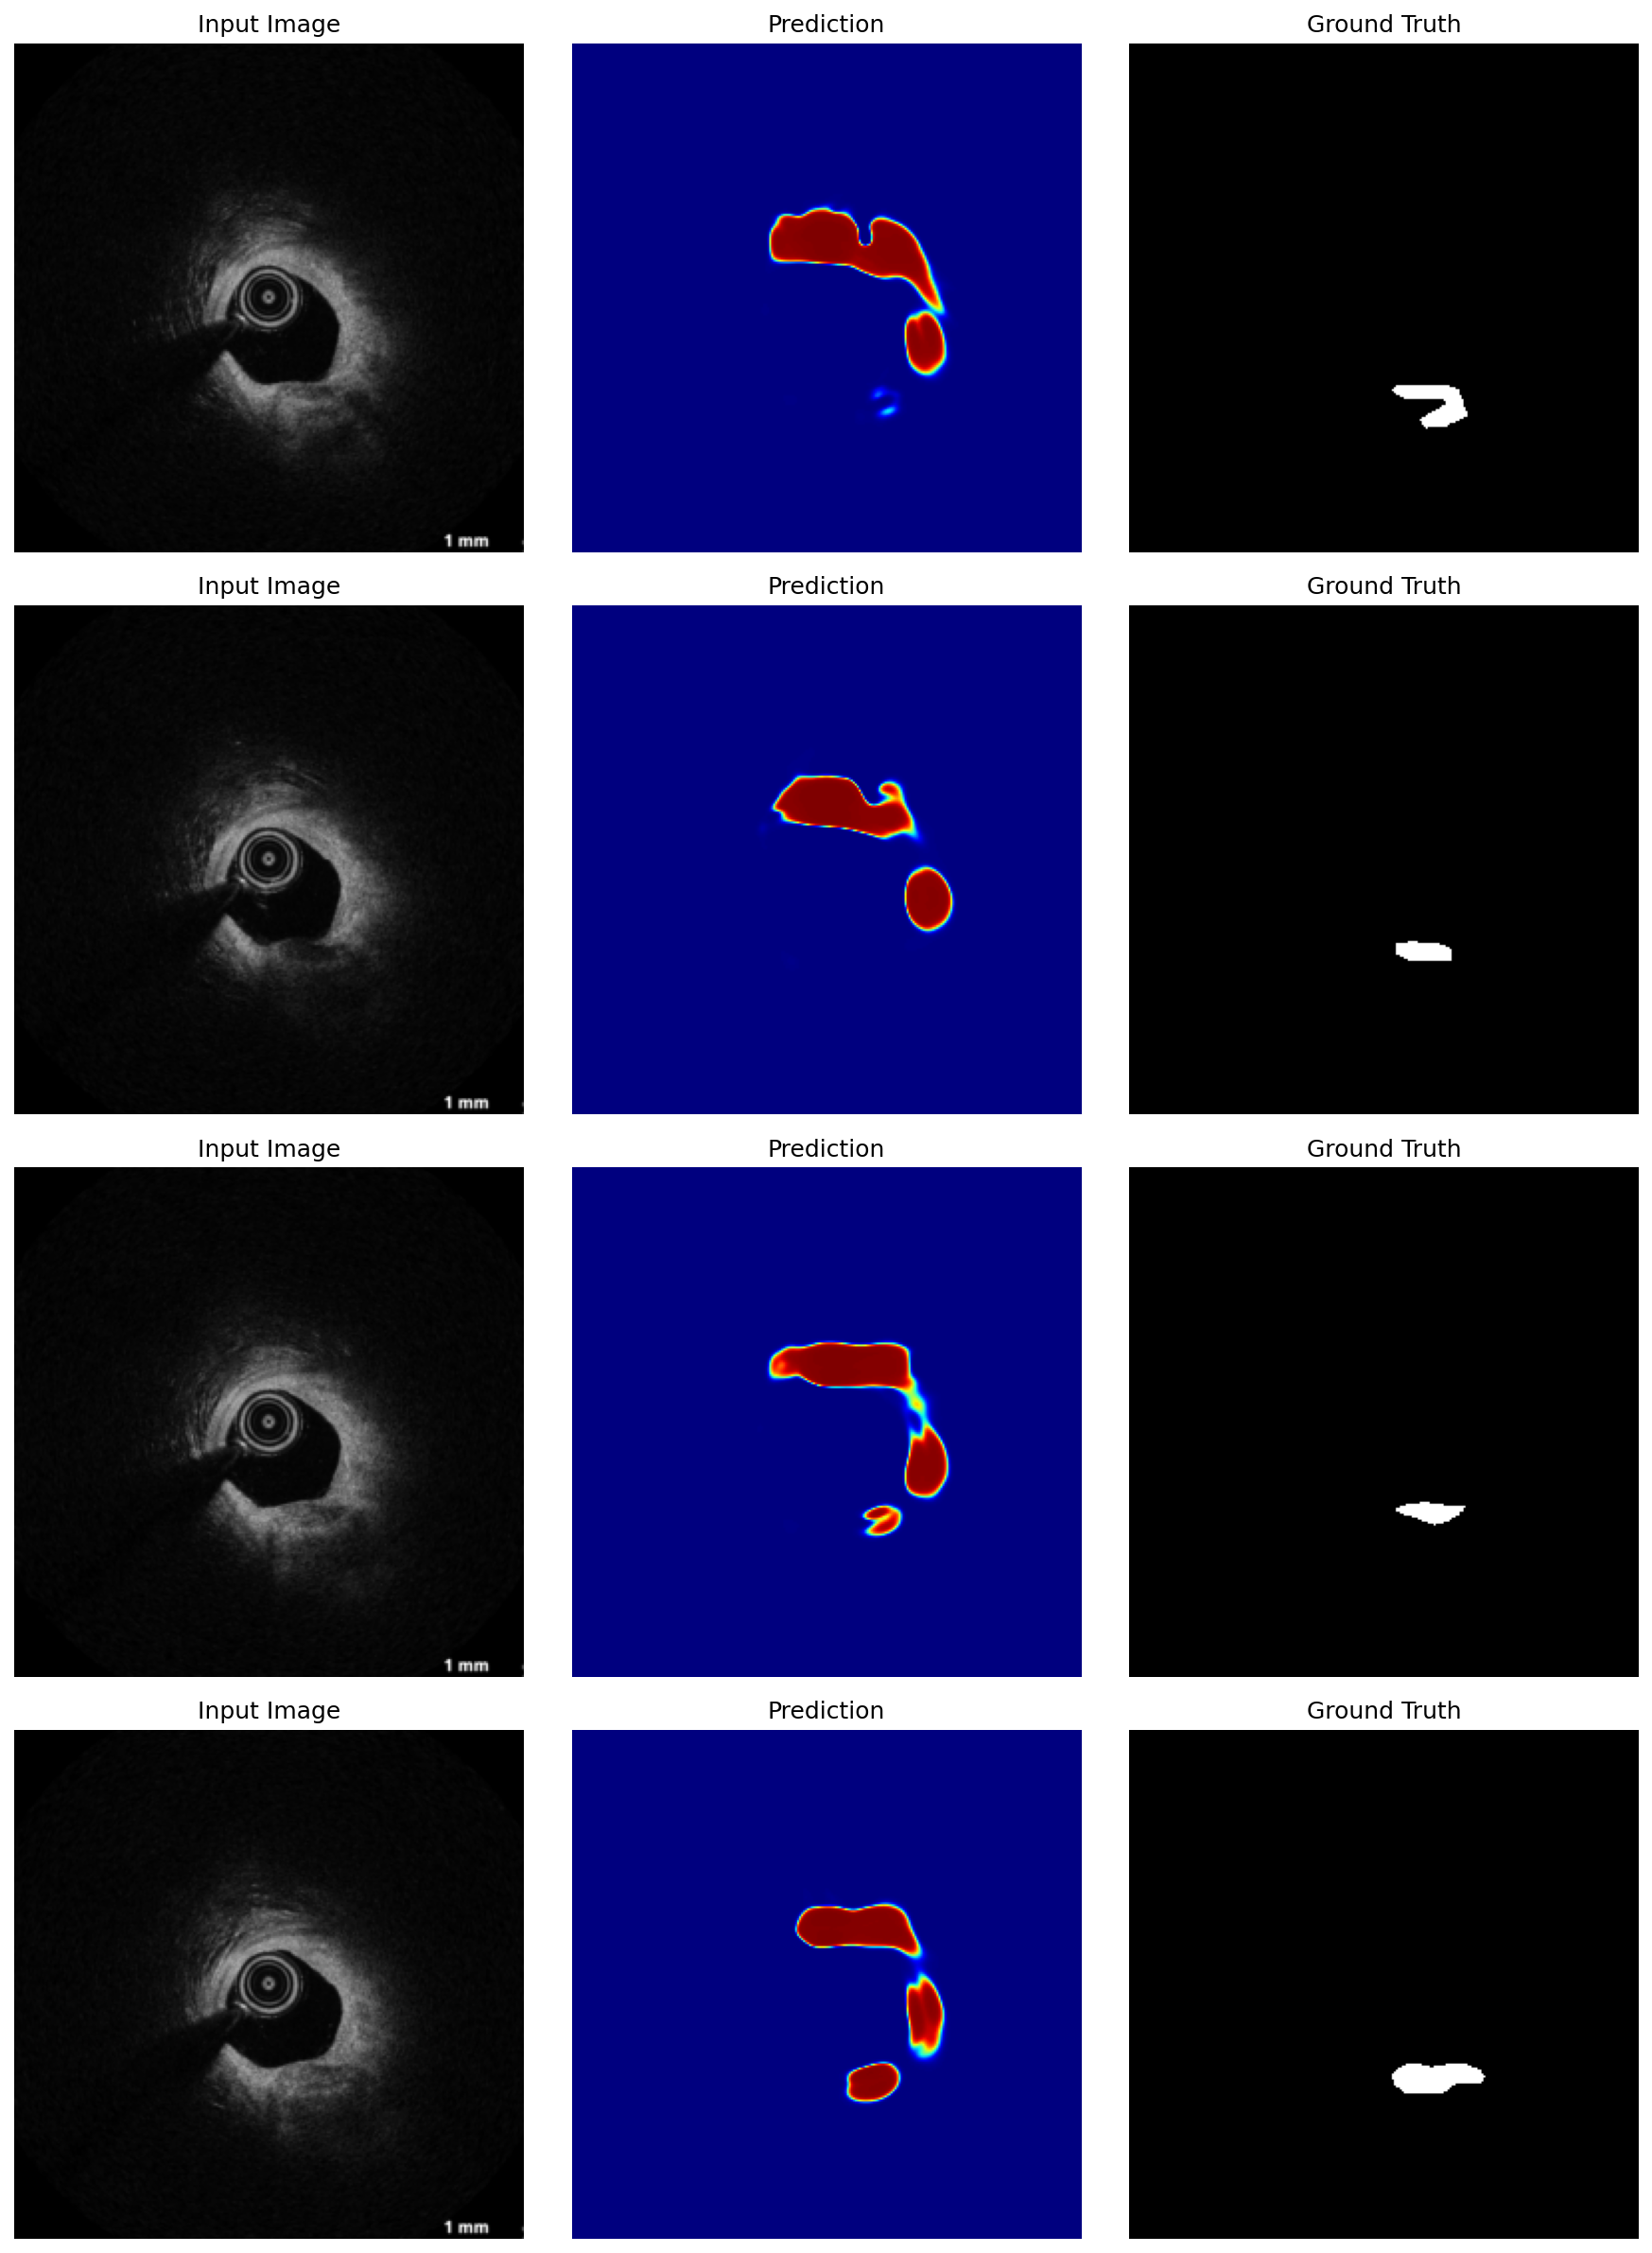
\includegraphics[width=\linewidth]{fold_1_best_epoch_168.png}
  \caption{Fold 1, val=P002, Dice=0.2861}
\end{subfigure}

\vspace{0.8em}

\begin{subfigure}{0.48\textwidth}
  \centering
  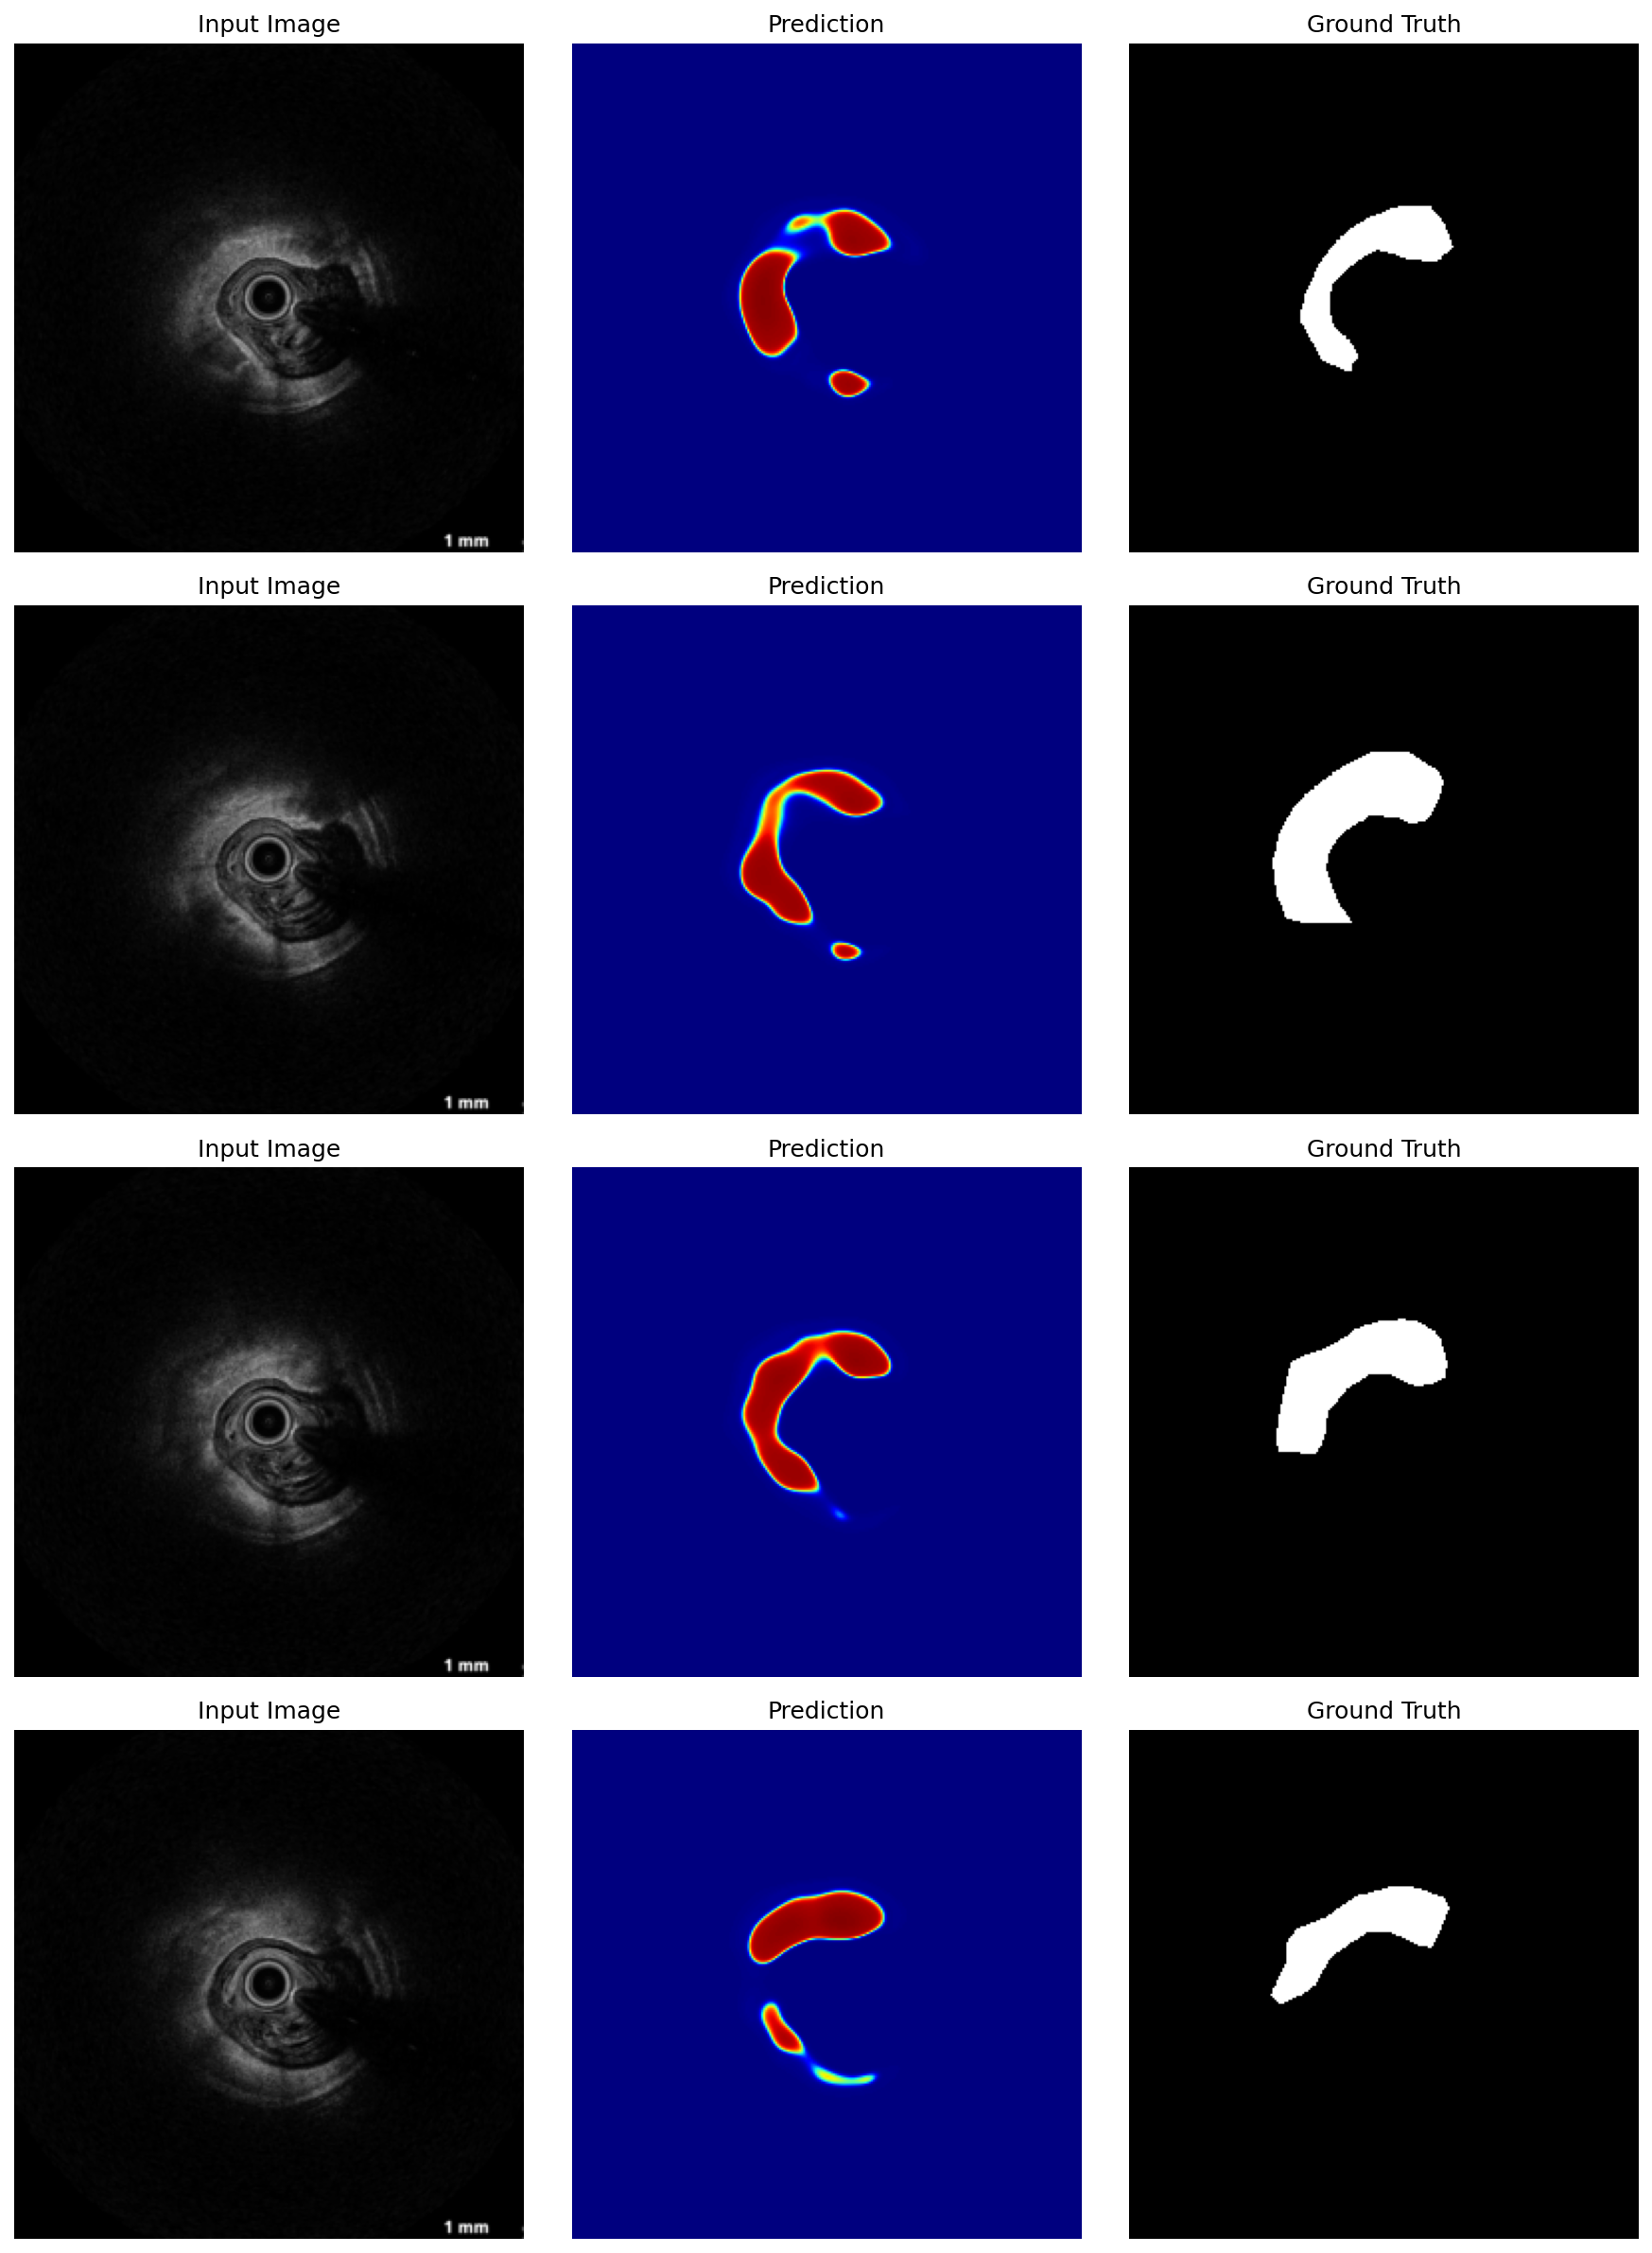
\includegraphics[width=\linewidth]{fold_2_best_epoch_052.png}
  \caption{Fold 2, val=P003, Dice=0.6323}
\end{subfigure}
\hfill
\begin{subfigure}{0.48\textwidth}
  \centering
  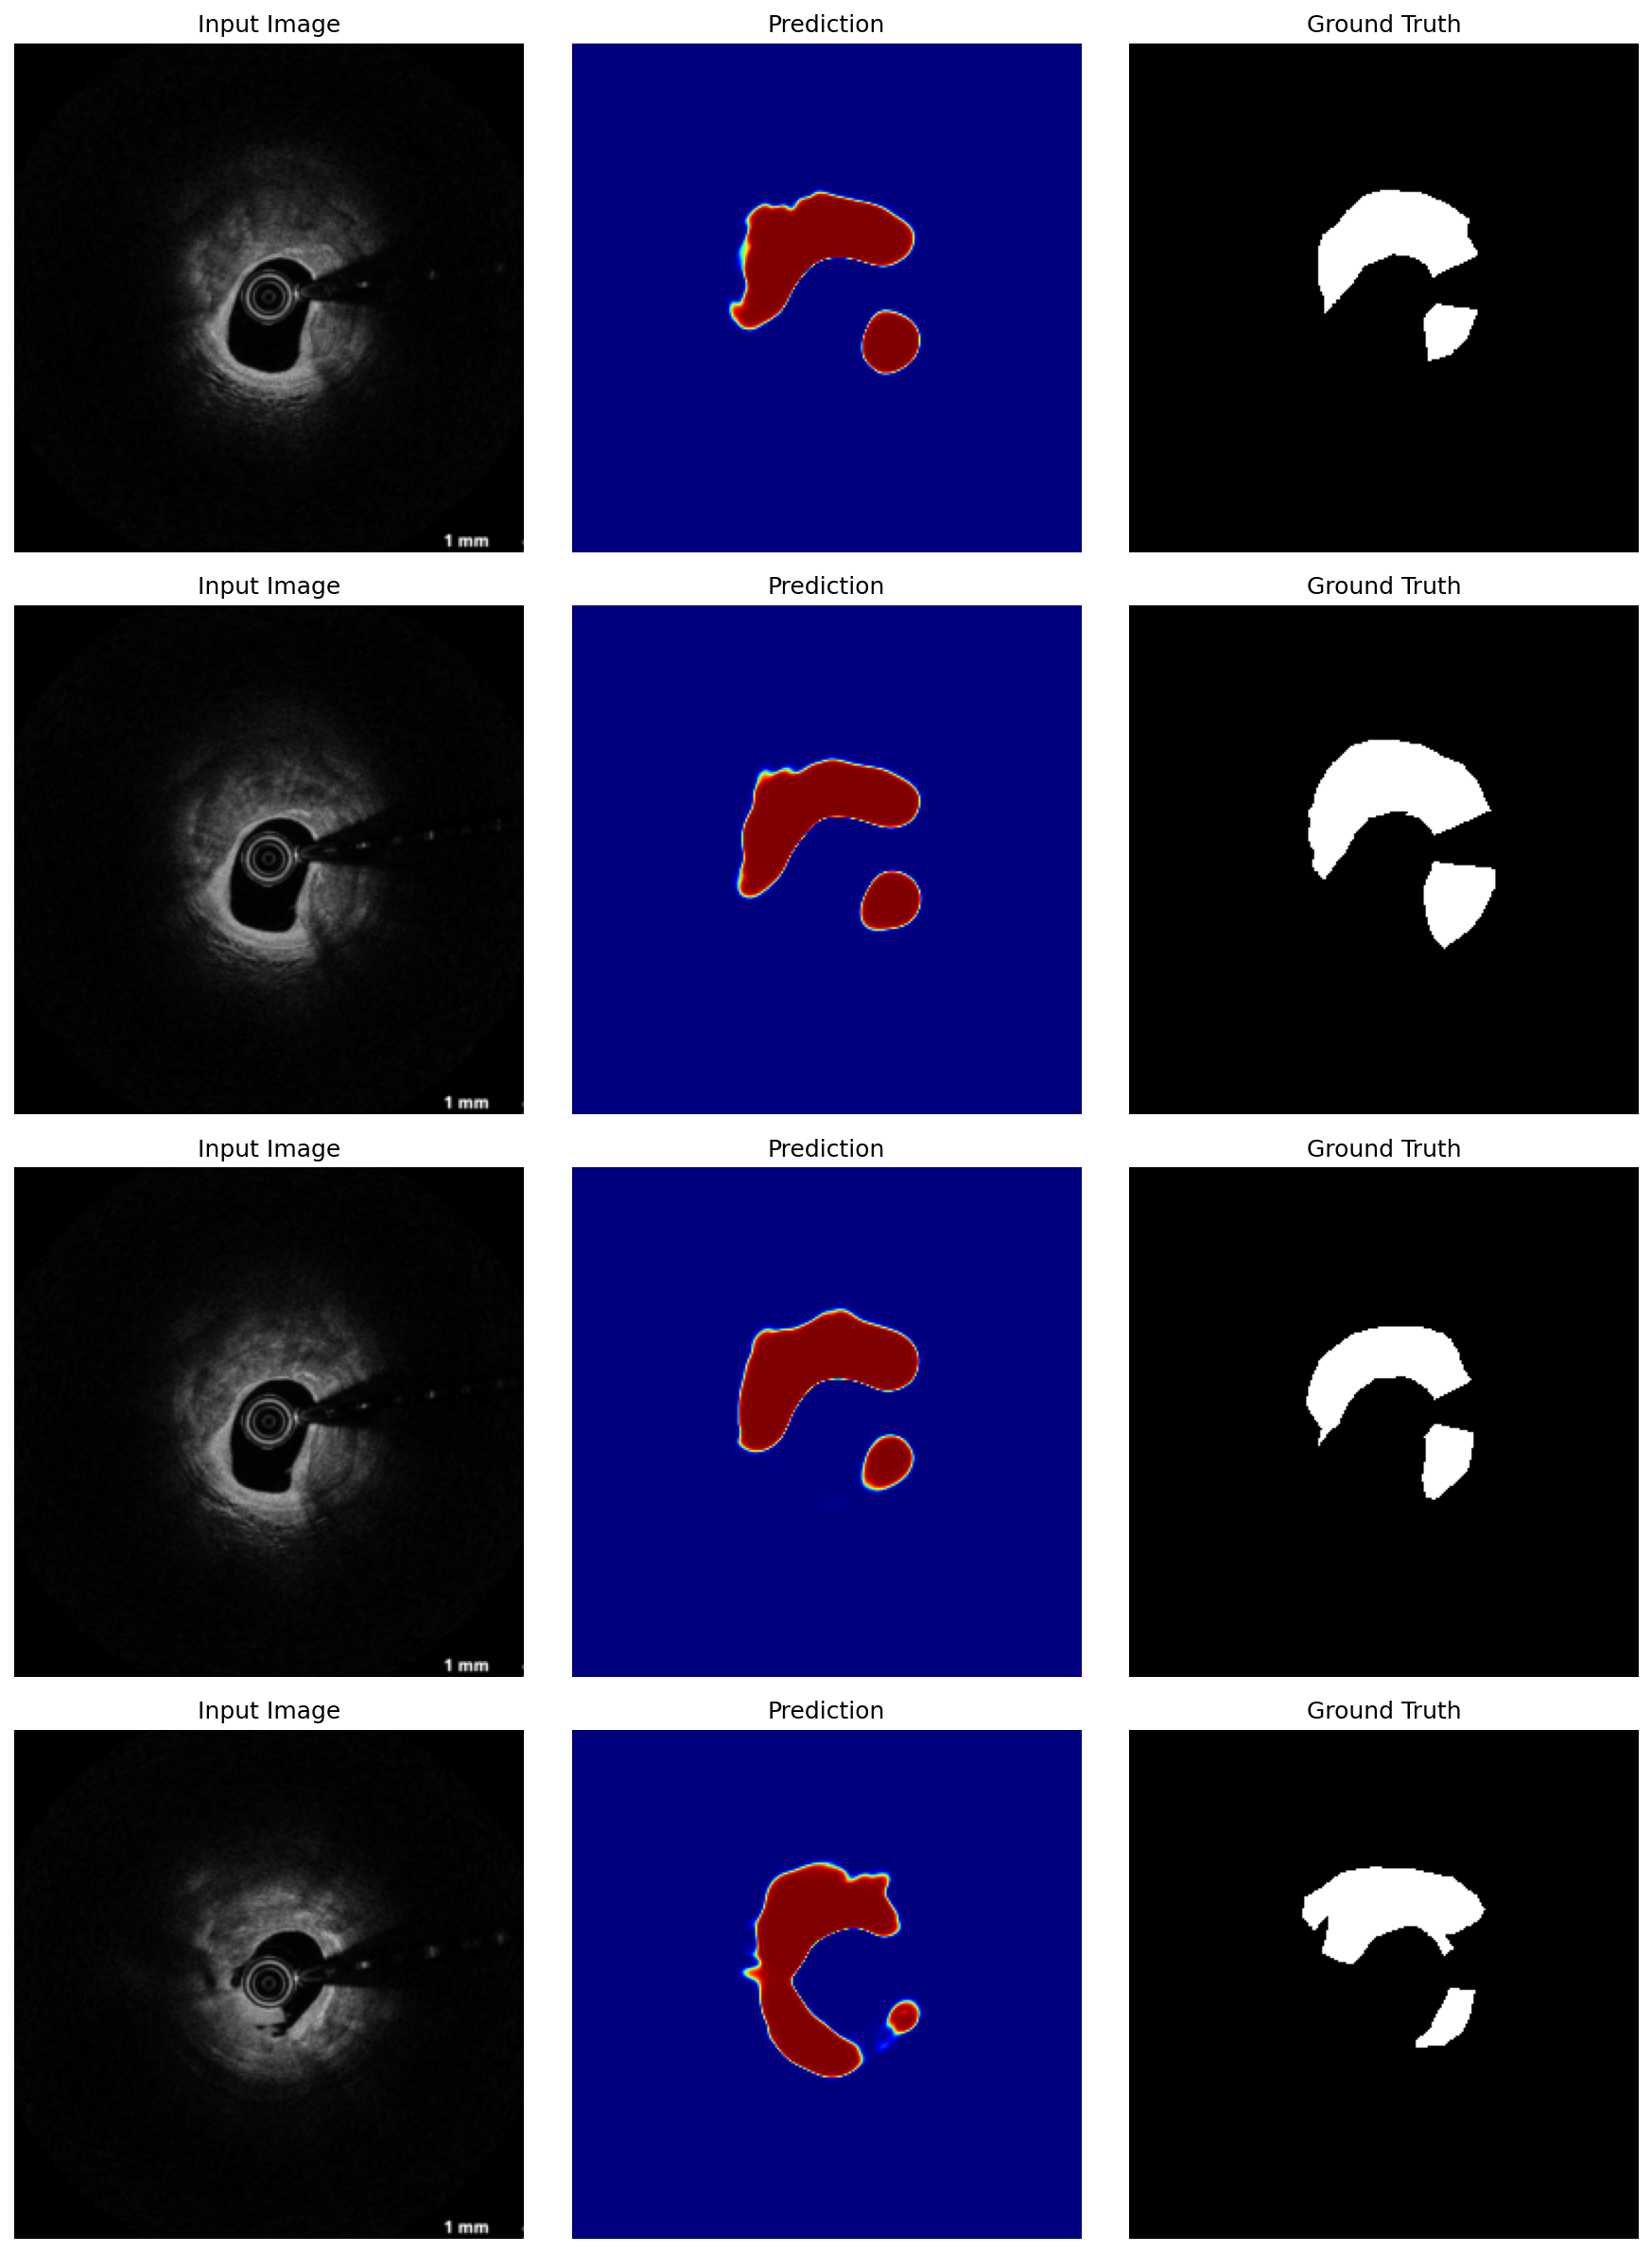
\includegraphics[width=\linewidth]{fold_3_best_epoch_094.png}
  \caption{Fold 3, val=P004, Dice=0.6374}
\end{subfigure}
\caption{Baseline 各 fold 的 best epoch 可视化结果。}
\label{fig:fold-vis}
\end{figure}

从可视化可以看出，模型在部分患者上能够定位到较合理的钙化区域；但在 P002 上，
预测区域与标注区域的一致性较差，存在明显患者间泛化波动。

\section{阈值扫描结果}

为了确认当前结果是否受二值化阈值影响，本阶段对 reproduced baseline checkpoints
进行了阈值扫描。扫描阈值为 0.3、0.4、0.5、0.6、0.7。

\begin{table}[htbp]
\centering
\caption{统一阈值下的全局 Mean Dice}
\label{tab:threshold-global}
\begin{tabular}{cc}
\toprule
统一阈值 & Mean Dice \\
\midrule
0.3 & 0.5213 \\
0.4 & 0.5169 \\
0.5 & 0.5124 \\
0.6 & 0.5091 \\
0.7 & 0.5032 \\
\bottomrule
\end{tabular}
\end{table}

全局最优统一阈值仍为 0.3。虽然部分 fold 的单折最优阈值不同，但统一阈值调整并未带来
整体提升。

\begin{table}[htbp]
\centering
\caption{每折最优阈值}
\label{tab:threshold-fold}
\begin{tabular}{cccc}
\toprule
Fold & 验证患者 & 单折最优阈值 & 单折最优 Dice \\
\midrule
0 & P001 & 0.3 & 0.5292 \\
1 & P002 & 0.7 & 0.2895 \\
2 & P003 & 0.3 & 0.6323 \\
3 & P004 & 0.6 & 0.6384 \\
\midrule
\multicolumn{2}{r}{全局统一最优阈值} & 0.3 & 0.5213 \\
\bottomrule
\end{tabular}
\end{table}

P002 的单折最优阈值为 0.7，但 Dice 仅从约 0.2864 提升到 0.2895，提升幅度很小。
这说明 P002 的主要问题不是简单阈值选择，而是模型输出的目标形态和患者分布差异。

\section{补充实验与未采用方案}

围绕最弱折 P002，本阶段验证过若干补充方案。这些方案对理解误差有帮助，但没有成为
当前正式主线。

\begin{table}[htbp]
\centering
\caption{补充实验结果}
\label{tab:extra-experiments}
\begin{tabular}{p{0.30\textwidth}p{0.24\textwidth}p{0.34\textwidth}}
\toprule
方案 & 关键结果 & 是否采用 \\
\midrule
全局连通域后处理 & P002 可提升，但 P003/P004 明显下降 & 不采用 \\
Focal alpha=0.5 & P002 Dice=0.2762 & 不采用，低于 baseline \\
BN + early stopping & P002 Dice=0.2409 & 不采用，明显低于 baseline \\
Focal Tversky + BN + early stopping & P002 LOPO Dice=0.3223；全局 Mean Dice=0.4561 & 不采用，改善 P002 但损害整体 \\
\bottomrule
\end{tabular}
\end{table}

其中 Focal Tversky + BN + early stopping 对 P002 有一定帮助，但会显著降低 P001 与
P003 的表现，使全局 Mean Dice 降至 0.4561。因此该方案更像是针对当前最弱患者的
局部调整，而不是稳健的全局配置。

\section{阶段性结论}

当前阶段最重要的结论如下：

\begin{itemize}
  \item reproduced baseline 是目前全局最优方案，Mean Dice 为 $0.5212 \pm 0.1424$；
  \item 统一阈值 0.3 是当前最合适的全局二值化阈值；
  \item P002 是当前最弱折，但专门优化 P002 会损害整体表现；
  \item 在剩余 14 名患者数据到位前，继续围绕现有 4 名患者深度调参的收益有限；
  \item 当前 baseline 可作为后续新增患者实验的对照基线。
\end{itemize}

因此，建议当前阶段保留 \textbf{MAE encoder + Conv decoder reproduced baseline}
作为正式 baseline。待剩余 14 名患者加入后，再重新进行 patient-level 泛化评估、
LOPO-CV 和必要的训练策略调整。

\section{结果包文件说明}

本结果包包含报告、图片、结果文件和关键代码配置。表~\ref{tab:file-index}
列出本 PDF 中提到的主要文件及其在结果包中的相对位置。

\begin{longtable}{p{0.28\textwidth}p{0.62\textwidth}}
\caption{结果包文件索引}
\label{tab:file-index}\\
\toprule
类型 & 相对路径 \\
\midrule
\endfirsthead
\toprule
类型 & 相对路径 \\
\midrule
\endhead
LaTeX 主文件 & \texttt{main.tex} \\
PDF 占位说明 & \texttt{pdf/PDF\_PLACEHOLDER.txt} \\
Fold 0 可视化 & \texttt{figures/fold\_0\_best\_epoch\_177.png} \\
Fold 1 可视化 & \texttt{figures/fold\_1\_best\_epoch\_168.png} \\
Fold 2 可视化 & \texttt{figures/fold\_2\_best\_epoch\_052.png} \\
Fold 3 可视化 & \texttt{figures/fold\_3\_best\_epoch\_094.png} \\
LOPO 结果 JSON & \texttt{data/results\_lopo\_20260424\_004401.json} \\
Checkpoint 摘要 & \texttt{data/checkpoint\_summary.json} \\
阈值扫描摘要 & \texttt{data/threshold\_sweep\_summary\_20260424\_baseline.json} \\
阶段决策记录 & \texttt{data/seg\_best\_decision\_20260424.md} \\
Review pack manifest & \texttt{data/manifest.json} \\
分割配置文件 & \texttt{code/config\_seg.py} \\
分割训练脚本 & \texttt{code/train\_seg.py} \\
分割模型定义 & \texttt{code/seg\_model.py} \\
数据集定义 & \texttt{code/ivoct\_seg\_dataset.py} \\
损失函数 & \texttt{code/seg\_losses.py} \\
评价指标 & \texttt{code/seg\_metrics.py} \\
\bottomrule
\end{longtable}

\end{document}
